% !TEX program = xelatex
\documentclass[a4paper,12pt]{article}
\usepackage{amsthm}
\usepackage{amssymb}
\usepackage{bm}
\usepackage{mathtools}
\usepackage[x11names]{xcolor}
\usepackage{xparse}
\usepackage{fontspec}
\usepackage{unicode-math}
\setromanfont[Ligatures={Common,Rare}]{DovesType-Regular.otf}
\setsansfont{Andika}
\setmathfont{Asana Math}[Scale=1]
\newfontfamily\TrajanP[Scale=1.0]{TRAJANPRO-REGULAR.OTF}
% \newfontfamily\TrajanP[Scale=1.0]{Tork}

% \usepackage{pstricks}
\usepackage{varwidth}
\usepackage{siunitx}
\usepackage{graphicx}
\usepackage[margin=1.5cm,top=1.5cm]{geometry}
\usepackage[most]{tcolorbox}
\usepackage{pgfplots}
\pgfplotsset{compat=newest}
\tcbuselibrary{skins,xparse,poster,breakable}
% \usetikzlibrary{fadings}
\usetikzlibrary{calc,math, plotmarks, shapes, shapes.geometric, positioning, angles, intersections, quotes, through, patterns, turtle, arrows.meta}
\usetikzlibrary{decorations.markings,backgrounds}
% \usepackage{etoolbox}
\usepackage{tkz-euclide}
\usepackage{xfrac}
% \usepackage{xlop}
% \newcommand\hole[2]{#1}  % for use with xlop
\pagenumbering{gobble}
%%%%%%%%%%%%%%%%%%%%%%%%%%%%%%%%%%%%%%%%%%%%%%%%%%%%%%%%%
\newcommand\markangle[9]{% origin X Y radius radiusmark mark colour opacity
%  % fill red circle offset-from-centre
  \begin{scope}
    \path[clip] (#1) -- (#2) -- (#3);
    \fill[color=#7,fill opacity=#8,draw=black,name path global=pcircle]  % global declaration required otherwise pcircle is not seen by the `named intersections=' lines below.
    (#1) circle (#4);
  \end{scope}
  % middle calculation
  \path[name path=line one] (#1) -- (#2);
  \path[name path=line two] (#1) -- (#3);
  \path[%
  name intersections={of=line one and pcircle, by={inter one}},
  name intersections={of=line two and pcircle, by={inter two}}
  ] (inter one) -- (inter two) coordinate[pos=#9] (place);
  % put mark
  \node at ($(#1)!#5!(place)$) {\scriptsize{#6}};
}
%%%%%%%%%%%%%%%%%%%%%%%%%%%%%%%%%%%%%%%%%%%%%%%%%%%%%%%%
\newcommand\tcircle[6]{% centre coord (x,y), radius, points, radpoint, colour, edge
  \coordinate (O) at (#1,#2); % centre of the circle
  \def\radius{#3}          % radius of the circle
  \def\npts{#4}            % number of the points
  \def\radpt{#5}           % radius of the points
  \colorlet{ptcolour}{#6}  % colour of the points
  % \draw (O) circle (\radius);
  \foreach \numpoint in {1,...,\npts}{
    \fill[ptcolour] (O) ++ (360/\npts*\numpoint:\radius) coordinate (C\numpoint) circle(\radpt);
  }
}

% \newcommand{\condSoln}[2]{\ifcsdef{r@#1}{#2}{}}

% \newcommand\fadingtext[3][]{%
%    \begin{tikzfadingfrompicture}[name=fading letter]
%      \node[text=transparent!0,inner xsep=0pt,outer xsep=0pt,#1] {#3};
%    \end{tikzfadingfrompicture}%
%    \begin{tikzpicture}[baseline=(textnode.base)]
%      \node[inner sep=0pt,outer sep=0pt,#1](textnode){\phantom{#3}};
%      \shade[path fading=fading letter,#2,fit fading=false]
%      (textnode.south west) rectangle (textnode.north east);%
%    \end{tikzpicture}%
% }

\definecolor{JISpurple}{RGB}{89,72,122}
\definecolor{JISivory}{RGB}{241,234,221}
\definecolor{JIStaupe}{RGB}{183,156,154}
\definecolor{PaleGreen}{RGB}{240,255,240} % 'Honeydew'

\AddToHook{shipout/background}{%
    \put (0in,-\paperheight){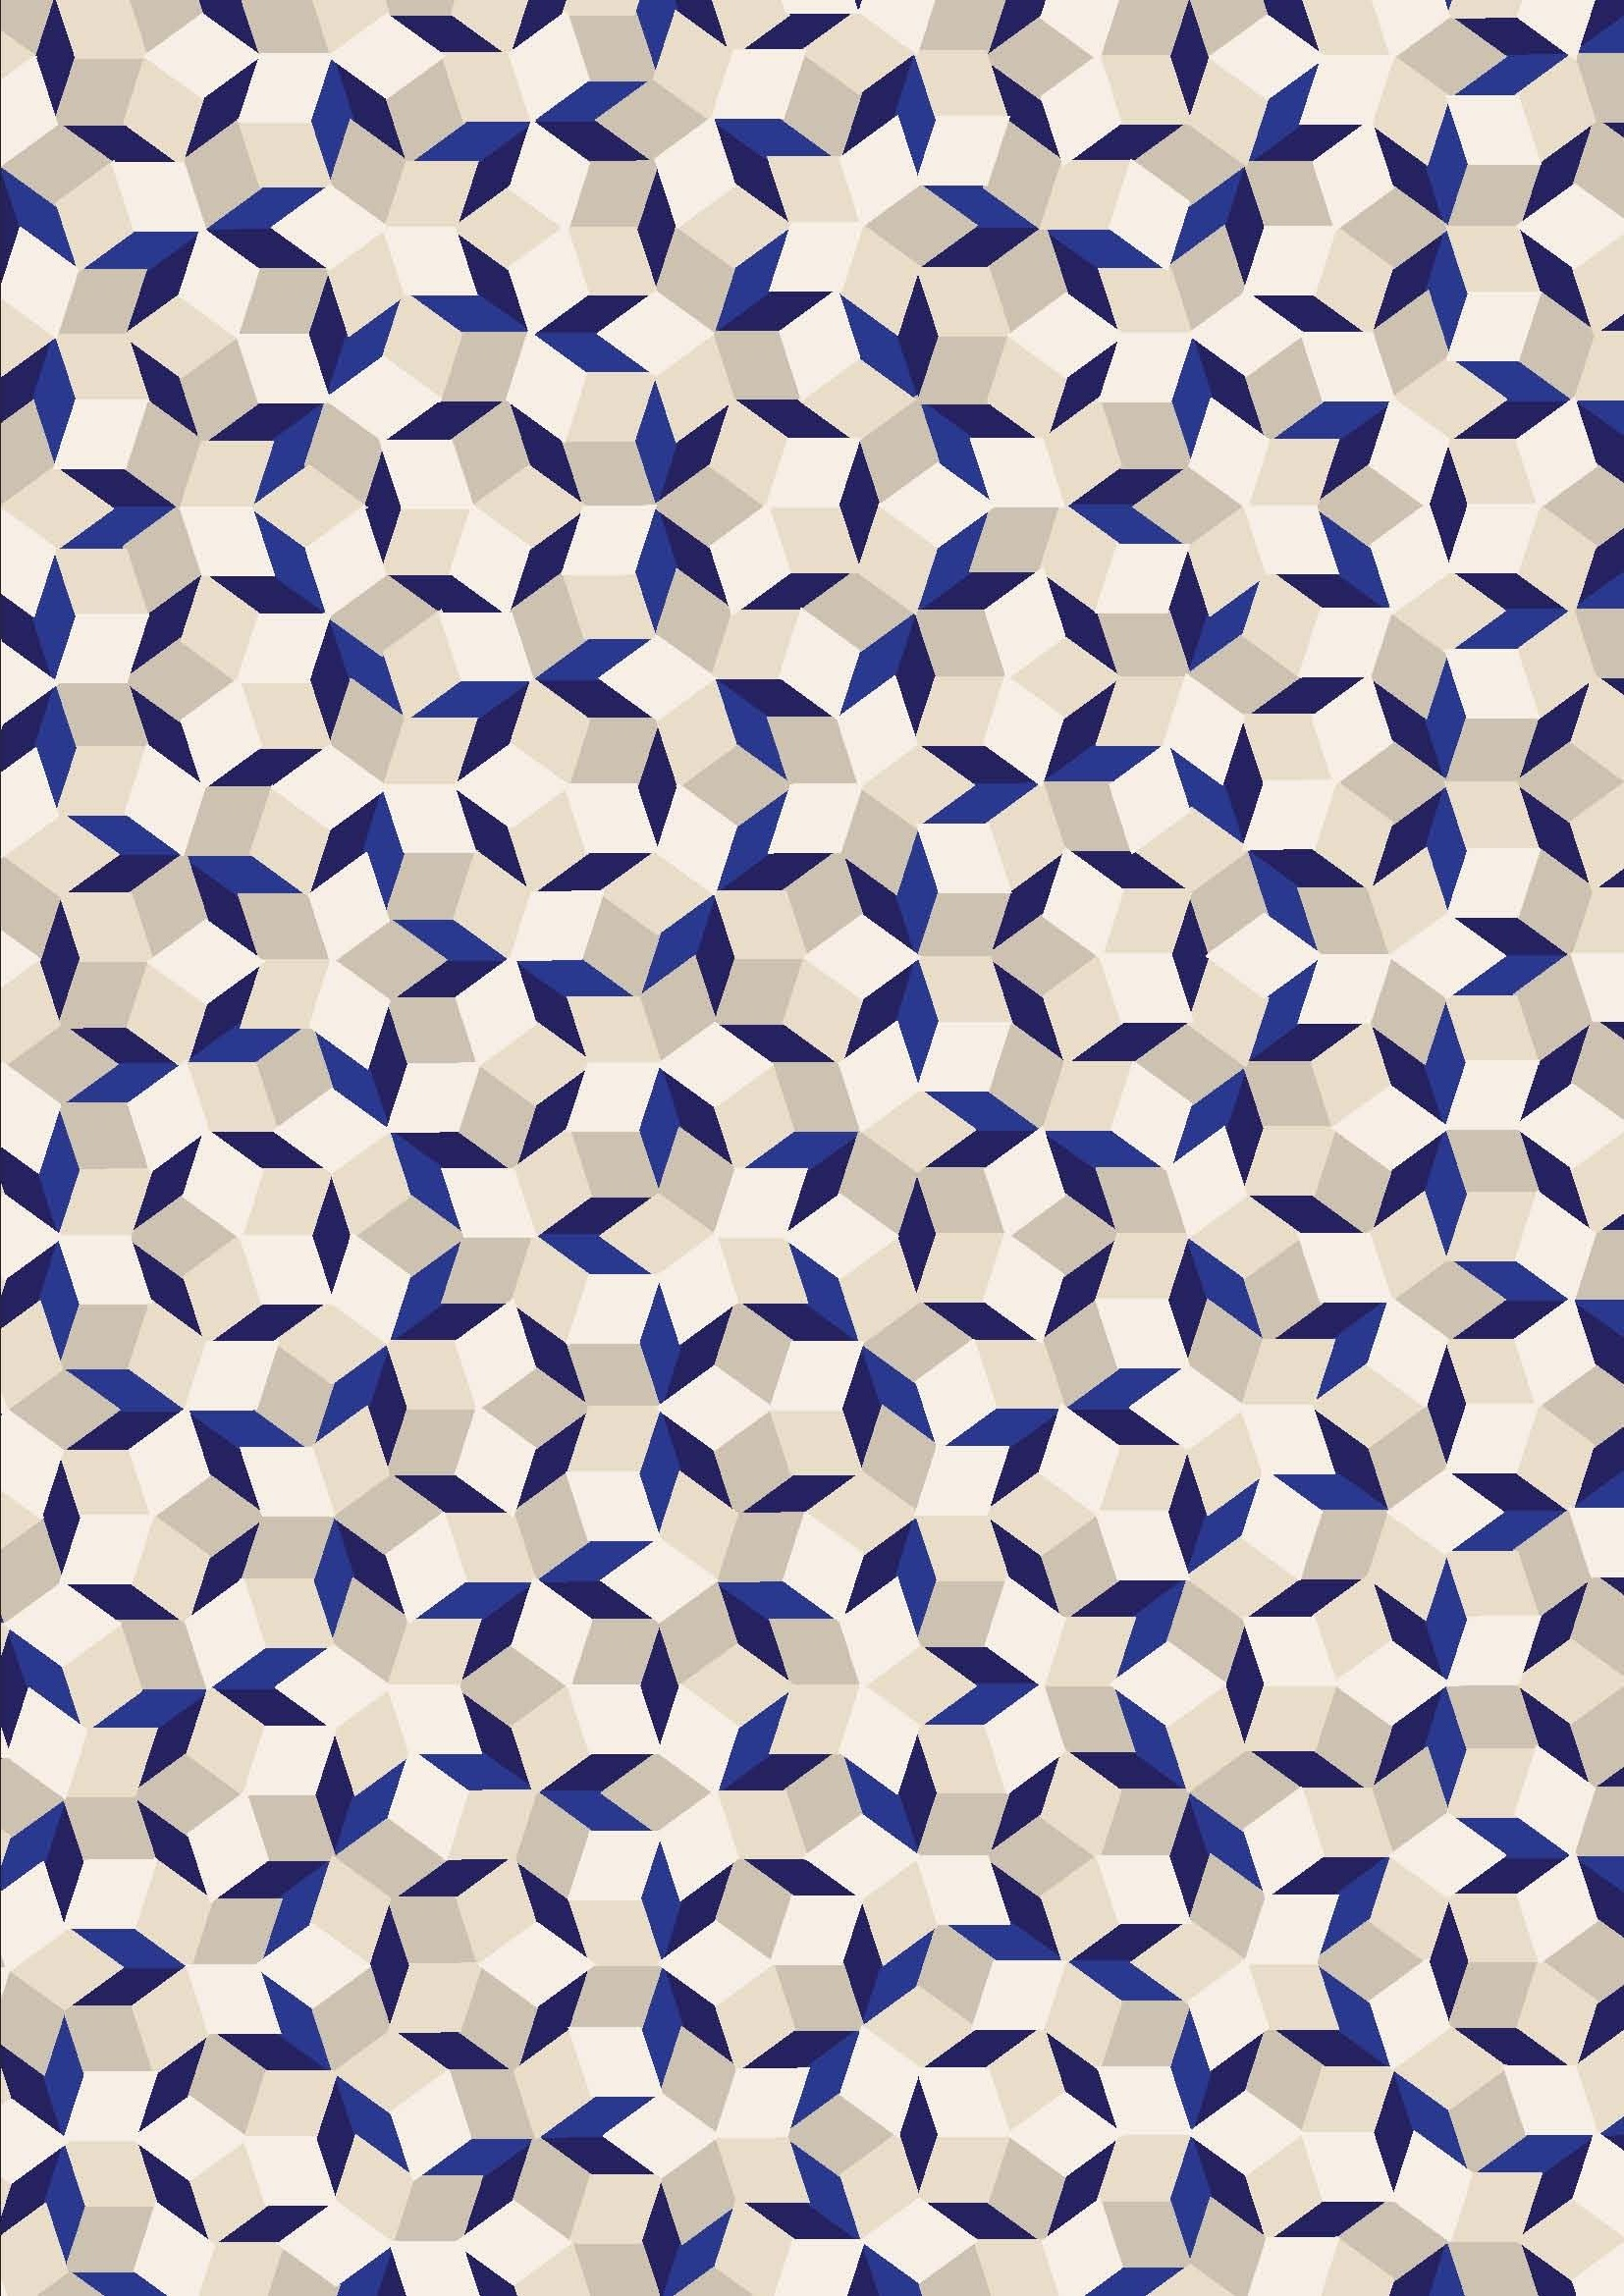
\includegraphics[width=\paperwidth,height=\paperheight]{images/penrose2r.jpg}}%
}

\newcommand\numberthis{\addtocounter{equation}{1}\tag{\theequation}}

\newtcolorbox{MyOuterBox}{%
  enhanced,
  % watermark graphics=images/santa_faces_watermark.jpg,
  % watermark opacity=0.8,
  % watermark zoom=2.0,
  breakable,
  frame style=JISpurple,
  colback=JISivory,
  colframe=JISpurple,
  title={
\includegraphics[width=0.9cm,height=0.9cm]{images/JIS Final Logo FA-02.png}\raisebox{3mm}{\Large{Maths Challenge}\hspace{18.8em} \Large{\bfseries\sffamily 23}}},
}

\newtcolorbox{MyInnerBox}[2][]{enhanced,%empty,
coltitle=JISpurple,colback=white,
breakable,
fonttitle=\bfseries\sffamily,
attach boxed title to top left={yshift=-1.5mm},
boxed title style={empty, size=small, top=1mm, bottom=0pt},
varwidth boxed title=0.5\linewidth,
frame code={
  \path (title.east|-frame.north) coordinate (aux);
\path[draw=JISpurple, line width=0.5mm, rounded corners,fill=white]
(frame.west) |- ([xshift=-2.5mm]title.north east) to[out=0, in=180] ([xshift=7.5mm]aux)-|(frame.east)|-(frame.south)-|cycle;
},
title={#2},#1}

\newtcolorbox{MyInnerSplitBox}[2][]{enhanced,%empty,
bicolor,sidebyside,sidebyside align=top seam,
righthand width=7.0cm,colbacklower=white,
sidebyside gap=5mm,
breakable,
coltitle=JISpurple,colback=white,
fonttitle=\bfseries\sffamily,
attach boxed title to top left={yshift=-1.5mm},
boxed title style={empty, size=small, top=1mm, bottom=0pt},
varwidth boxed title=0.5\linewidth,
frame code={
  \path (title.east|-frame.north) coordinate (aux);
\path[draw=JISpurple, line width=0.5mm, rounded corners,fill=white]
(frame.west) |- ([xshift=-2.5mm]title.north east) to[out=0, in=180] ([xshift=7.5mm]aux)-|(frame.east)|-(frame.south)-|cycle;
},
title={#2},#1}


\newtcolorbox{MySolutionBox}[1][]{%
  enhanced,
  breakable,
  frame style=JISpurple,
  colback=PaleGreen, colframe=green,
  title={\Large Solution},
  drop fuzzy shadow,
  halign=left,
  #1
}

%%%%%%%%%%%%%%%%%%%%%%%%%%%%%%%%%%%%%%%%%%%%%%%%%%
\newtoggle{SOLUTION}
%%% Uncomment the appropriate line below to show solutions %%%
% \toggletrue{SOLUTION}
\togglefalse{SOLUTION}
%%%%%%%%%%%%%%%%%%%%%%%%%%%%%%%%%%%%%%%%%%%%%%%%%


%%%%%%%%%%%%%%%%%%%%%%%%%%%%%%%%%%%%%%%%%%%%%%%%%%
%%%%%%            DOCUMENT BEGINS           %%%%%%
%%%%%%%%%%%%%%%%%%%%%%%%%%%%%%%%%%%%%%%%%%%%%%%%%%
\begin{document}


  \begin{MyOuterBox}
    \iftoggle{SOLUTION}{Here are the full, or partial solutions.
    }{
      Welcome to this week's Maths Challenge!\\
      Have a go at both questions!\\
      Drop your solution in the box in the staffroom by Tuesday.
    }
       \begin{MyInnerBox}{Year 8 and below}
     The pages of a book are numbered; \(1,\;2,\;3,\ldots\)\par
     It takes \(852\) digits to number all the pages of the book.\par
     What is the number of the last page of the book?\par
      \iftoggle{SOLUTION}{%conditional output begin
      \begin{MySolutionBox}
        From page 1 to page 9 we need \(9\) digits.\par
        From page 10 to page 99 we need \(90\times 2=180\) digits. \(189\) digits in total so far.\par
        We have \(852-189=663\) digits left, and we have up to page 99 so far.\par
        From page 100 to page 999 we would need \(900\times 3=2700\) digits.\par
        With \(663\) digits we can number \(663\div 3=221\) three-digit pages.\par
        Starting with page \(100\) that means we would reach page \(220\).
      \end{MySolutionBox}
    }{}%conditional output end
    \end{MyInnerBox}


    \vspace{0.4cm}
          \begin{MyInnerBox}{Year 9 and above}
        How many set of three positive integers, \(a,\;b,\;c\) satisfy the following two conditions simultaneously?\par
        \begin{align}
          6ab &= c^{2}\\
          a<b<c&\leq 35
        \end{align}
      \iftoggle{SOLUTION}{%conditional output begin
      \begin{MySolutionBox}
        We see from the second condition that the three integers must be different.\par
        From the first condition we can see that \(c\) must be a multiple of \(6\).\par
        So \(c\) could be \(6,\;12,\;18,\;24\) or \(30\).\par
        Now we need \(a\) and \(b\) such that \(a\times b=\frac{c^{2}}{6}\). Let's look at the possibilities.\par
        \begin{tabular}{l|c|c|c|c|c|l}
          No. & \(c\) & \(c^{2}\) & \(\sfrac{c^{2}}{6}\) & \(a\) & \(b\) &\\\hline
          \(1\) & \(6\) & \(36\) & \(6\) & \(2\) & \(3\) & Solution\\
          \(2\) & \(12\) & \(144\) & \(24\) & \(2\) & \(12\) & Two digits the same, not a solution\\
          \(3\) & " & " & \(24\) & \(3\) & \(8\) & Solution\\
          \(4\) & " & " & \(24\) & \(4\) & \(6\) & Solution\\
          \(5\) & \(18\) & \(324\) & \(56\) & \(4\) & \(14\) & Solution\\
          \(6\) & " & " & \(56\) & \(7\) & \(8\) & Solution\\
          \(7\) & \(24\) & \(576\) & \(96\) & \(6\) & \(16\) & Solution\\
          \(8\) & " & " & \(96\) & \(8\) & \(12\) & Solution\\
          \(9\) & \(30\) & \(900\) & \(150\) & \(6\) & \(25\) & Solution\\
          \(10\) & " & " & \(150\) & \(10\) & \(15\) & Solution
        \end{tabular}\par\medskip
        So we have nine solutions, in triplets \((a,\;b,\;c)\) they are\\
        \((2,3,6),\;(3,8,12),\;(4,6,12),\;(4,14,18),\;(7,8,18),\)\\
        \((6,16,24),\;(8,12,24),\;(6,25,30),\;(10,15,30)\)\\
      \end{MySolutionBox}
    }{}%conditional output end
    \end{MyInnerBox}


  \end{MyOuterBox}

%%%%%%%%%%%%%%%%%%%%%%%%%%%%%%%%%%%%%%%%%%%%%%%%%%
\end{document}



